\section{Modulacja}

\subsection{Dlaczego potrzebujemy modulacji?}

Modulacja cyfrowa to technika zamiany bitów na sygnał oraz sygnału na bity. Jest kluczowym zagadnieniem w przesyle danych pomiędzy systemami komputerowymi. W odróżnieniu od modulacji analogowej, gdzie przesyłane dane wybierane są z przedziału,
modulacja cyfrowa operuje na dyskretnym zbiorze danych (bitach).

Dane reprezentowane są w postaci zmiany parametrów przesyłanego sygnału. Wyróżniane są cztery podstawowe metody:

\begin{enumerate}
    \item PSK (phase-shift keying) --- zmiana fazy fali nośnej sygnału,
    \item FSK (frequency-shift keying) --- zmiana częstotliwości fali nośnej sygnału,
    \item ASK (amplitude-shift keying) --- zmiana amplitudy fali nośnej sygnału,
    \item QAM (quadrature amplitude modulation) --- połączenie PSK oraz ASK, a więc zmieniana jest zarówno amplituda oraz faza.
\end{enumerate}

Zmiany sygnału (symbole) kodujące kolejne bity wybierane są ze skończonego zbioru nazywanego alfabetem modulacji.
Dział ten przedstawi popularne techniki modulacji w technologiach Ethernetowych.

\subsection{Wprowadzenie}

Aby ławiej zrozumieć ideę stojącą za bardziej skomplikowanymi technikami modulacji, należałoby na wprowadzeniu wyjaśnić kilka podstawowych pojęć.

Główną charakterystyką łącza jest szerokość pasma (ang. bandwidth) --- określa ona maksymalną (teoretyczną) liczbę bitów jaką łączę jest w stanie przesłać w danym czasie. Podawana jest ona w bitach na sekundę [$bps$] lub w hercach [Hz].

Przepustowość (ang. channel capacity) --- rzeczywista szerokość pasma, zmierzona w określonych warunkach.

Przepływność (ang. bit rate) --- rzeczywista ilość bitów transmitowanych w jednostce czasu poprzez kanał, podawana również w $bps$ lub Hz. Jest stałą charakterystyką danego łącza.

W 1924 roku Harry Nyquist przedstawił światu równanie, za pomocą którego określić można maksymalną przepływność łącza o szerokości pasma $B$ z wykorzystaniem $V$ poziomów:

\begin{align*}
    \text{Przepływność}_{max} &= 2B * log_{2}{V}
\end{align*}

24 lata później Claude Shannon rozszerzył równanie Nyquista, uwzględniając szum. Udowodnił on, że maksymalną przepływność łącza o szerokości pasma $B$ oraz stosunku sygnału do szumu $S/N$ można
obliczyć ze wzoru:

\begin{align*}
    \text{Przepływność}_{max} &= B * log_{2}{(1 + S/N)}
\end{align*}

Granica ta nazywana jest limitem Shannona.

Innym ważnym pojęciem jest multipleksacja (ang. multiplexing) i oznacza przesył wielu symboli jednocześnie w jednym kanale --- realizowany w postaci kilku przewodów, na które dane podawane są jednocześnie w każdym cyklu zegara.

\subsection{Non-Return-to-Zero}

Na początku rozważmy przykład. Najprostszą metodą byłoby używanie dodatniego napięcia dla bitu równego 1 i ujemnego napięcia dla 0.
Technika ta nosi nazwę \textbf{NRZ (Non-Return-to-Zero)}.
W praktyce wykorzystywana jest w połączeniu z kodowaniem liniowym np. 64b/66b, ale nie stosuje się tej techniki samoistnie.
Jest tak, ponieważ podczas przesyłania danych mogą wystąpić długie ciągi zer lub jedynek, a więc nadawany sygnał nie będzie się zmieniał.
Jest to zjawisko niepożądane podczas transmisji i może doprowadzić do desynchronizacji zegarów strony nadawczej i odbiorczej.

Rozważmy też przypadek, w którym nadawane jest naprzemiennie 1 i 0 --- otrzymamy wówczas okres równy 2 bity, co oznacza, że potrzebujemy pasma B/2 Hz przy prędkości B bit/s.
Nie trudno zauważyć, że do szybszego nadawnia zwiększona musi zostać szerokość pasma, co nie jest optymalnym rozwiązaniem z uwagi na ograniczoność tego zasobu \cite{Computer-networks-Tanenbaum}.

Jednym z rozwiązań tego problemu jest wykorzystanie większej ilości poziomów napięcia. W powyższym przykładzie zastosowane zostały dwa poziomy, a co za tym idzie mamy do dyspozycji dwa symbole przesyłane przez kanał.
Zwiększenie poziomów do 4 dałoby nam 4 różne symbole, a więc 2 bity informacji. W rezultacie przepływność wzrosła dwukrotnie, natomiast szerokość pasma nie zmieniła się. Technika zadziała pod warunkiem, że strona odbiorcza dysponuje sprzętem, który pozwoli jej na
rozróżnienie wielu poziomów napięcia. Jednakże w praktyce jest to koszt, który jesteśmy w stanie ponieść.

\subsection{Pulse-Amplitude Modulation}

Pulse-Amplitude Modulation (PAM) jest jedną z najpopularniejszych technik modulacji wykorzystywaną w technologiach Ethernetowych. Można ją również zobaczyć w innych technologiach (USB4, PCI Express 6.0). Jest to rodzaj modulacji, w którym dane przesyłane jako zmiany amplitudy sygnału. Modulacje PAM można podzielić na dwie kategorię:

\begin{enumerate}
    \item single polarity PAM --- do sygnału dodawana jest stała składowa, aby wartości napięcia były dodatnie
    \item double polarity PAM --- wartości mogą być ujemne lub dodatnie
\end{enumerate}

Modulacja PAM pozwala na przesył więcej niż jednego bitu w jednym takcie zegara, dzięki czemu zgodnie z równaniem Nyquista, zwiększona może zostać przepływność przy niezmienionej szerokości pasma.
Poszczególne techniki PAM różnią się między sobą liczbą wykorzystywanych poziomów modulacji (technika NRZ może zatem być nazwana PAM2).
Liczba możliwych poziomów jest nieograniczona, jednak wraz ze wzrostem liczby poziomów, różnica pomiędzy symbolami maleje --- a to utrudnia stronie odbiorczej odczyt symboli. Dlatego właśnie rodzaj modulacji PAM wybiera się na podstawie możliwości strony nadawczej i odbiorczej. W systemach wbudowanych czy technologiach automotive wykorzystywanych jest mniej poziomów,
ponieważ w tych przypadkach liczy się kompaktowość, a przepływ danych nie jest duży. Zupełnie odwrotnie jest w technologiach Gigabit Ethernet, gdzie nie ma tak restrykcyjnych ograniczeń sprzętowych, a danych do przesyłu jest dużo.

Warto zwrócić uwagę na to, że wykorzystanie większej ilości poziomów nie adresuje problemu długich sekwencji samych zer lub jedynek. Dlatego również tu
stosuje się mechaznizmy zamiany wprowadzonych danych na bardziej zróżnicowany ciąg (np. kodowanie liniowe, skrambling).

\subsubsection{PAM3}

PAM3 --- trzypoziomowa modulacja PAM --- do przesyłu wykorzystuje wartości $+1$, $0$, $-1$. Jeden symbol koduje $log_{2}{3} \approx 1,58 \text{ bit/symbol}$.
PAM3 użyty został m.in. w standardach 100BASE-T4 (wczesna implementacja Fast Ethernet) i BroadR-Reach Ethernet standard --- wykorzystywany w branży automotive, opracowany przez firmę Broadcom Corporation.
Nie jest to schemat modulacji PAM, który często pojawia się w praktycznych rozwiązaniach z uwagi na to, że technologie wykorzystujące tę technikę nie zostały szeroko przyjęte.

Ciekawym aspektem jest podział bitów na symbole. Na pierwszy rzut oka widać, że istnieje problem z grupowaniem bitów --- nie można przecież przesłać $1,58$ bita. W modulacjach z liczbą poziomów będącą potęgą $2$ podział jest bardzo prosty --- bity grupujemy w dwójki, czwórki\dots i bezpośrednio mapujemy na symbole.

Tutaj rozwiązaniem jest tymczasowa zamiana bitów na trity (system trójkowy). Przykładowo w wersji drugiej USB4 dane dzieli się 11-bitowe grupy, po czym każda z nich zamienana jest na 7 tritów, osiągając przy tym
efektywność rzędu $\frac{11/7}{log_{2}{3}} * 100\% \approx 99\% $


\subsubsection{PAM4}

PAM4 --- czteropoziomowa modulacja PAM --- do przesyłu wykorzystuje wartości $3$, $1$, $-1$, $-3$, które kolejno odpowiadają logicznym wartościom 11, 10, 01, 00. W porównaniu do NRZ (Non-Return-to-Zero) ma przewagę posiadania dwukrotnie większej przepływność przy tej samej prędkości transmisji, co ilustruje poniższy rysunek \cite{Intel-pam4}:

\begin{figure}[ht]
    \centering
    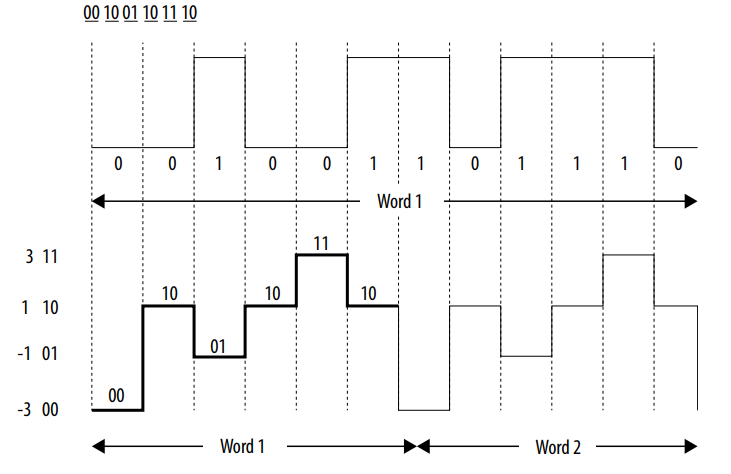
\includegraphics[width=\textwidth]{pam4_vs_nrz.png}
    \caption{Porównanie NRZ oraz PAM4}
    \label{fig:pam4_vs_nrz}
\end{figure}

Warto zwrócić uwagę na to, że w NRZ mamy jedno narastające zbocze ($0 \rightarrow 1$) i jedno opadające zbocze ($1 \rightarrow 0$), co daje dwie zmiany napięcia. W przypadku PAM4 jest to 6 narastających zbocz
($00 \rightarrow 01, 00 \rightarrow 10, 00 \rightarrow 11, 01 \rightarrow 10, 01 \rightarrow 11, 10 \rightarrow 11$) oraz 6 opadających zbocz
($11 \rightarrow 10, 11 \rightarrow 01, 11 \rightarrow 00, 10 \rightarrow 01, 10 \rightarrow 00, 01 \rightarrow 00$), które łącznie dają 12 różnych zmian napięcia.
Ma to znaczący wpływ na stosunek sygnału do szumu (SNR).

PAM4 stał się bardzo popularny w ostatnich latach i jest wykorzystywany m.in. w technologiach 100, 200 i 400 Gigabit Ethernet. Format ten został ustandaryzowany
także dla światłowodów (przykładowo 200GBASE-DR4).

\begin{figure}[ht]
    \centering
    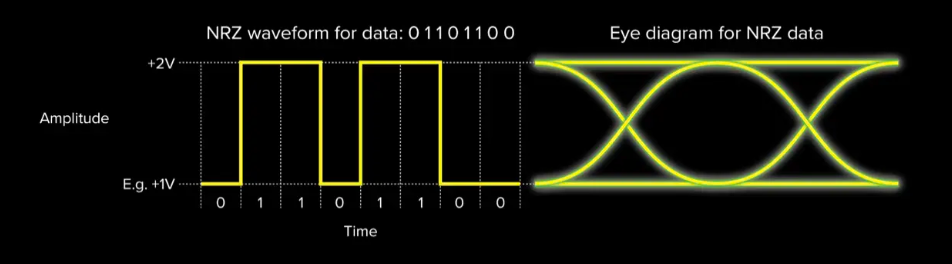
\includegraphics[width=\textwidth]{eye_diagram_nrz.png}
    \caption{Diagram oka NRZ}
    \label{fig:diagram_oka_nrz}
\end{figure}

\begin{figure}[ht]
    \centering
    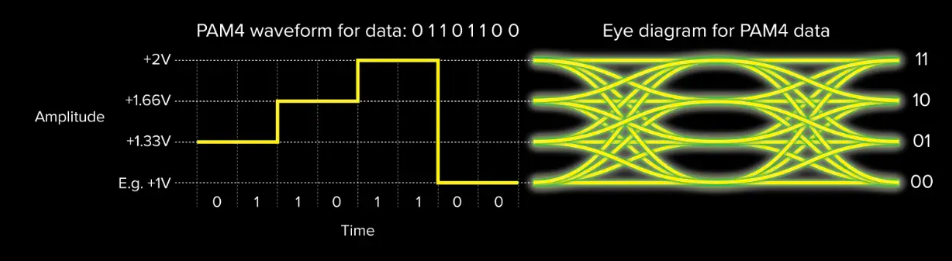
\includegraphics[width=\textwidth]{eye_diagram_pam4.png}
    \caption{Diagram oka PAM4}
    \label{fig:diagram_oka_pam4}
\end{figure}

\subsubsection{PAM5}
PAM5 --- pięciopoziomowa modulacja PAM --- wykorzystuje wartości $-2$, $-1$, $0$, $1$, $2$. PAM5 pojawiło się w 1000BASE-T, gdzie dane przesyłane są na czterech parach
skrętki jednocześnie. W technologii 1000BASE-T, do mapowania bitów na symbole wykorzystywana jest technika kodowania 8B1Q4, która zamienia
8 bitów na cztery pięciowartościowe symbole (4D-PAM4). Zauważyć można, że do takiej konwersji wystarczyłyby czterowartościowe symbole, jednakże
jeden nadmiarowy bit pomaga przesyłać słowa kontrolne.

\begin{figure}[ht]
    \centering
    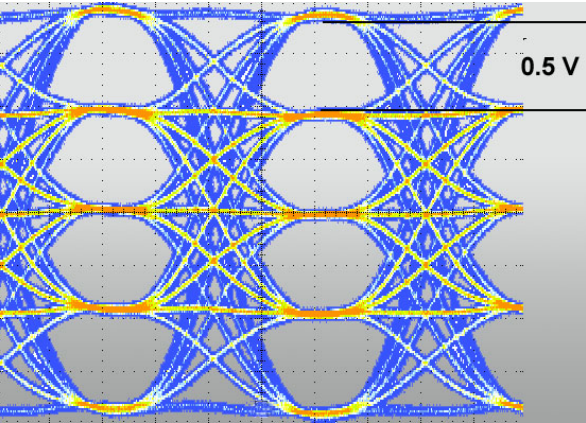
\includegraphics[width=\textwidth]{pam5_eye_diagram.png}
    \caption{Diagram oka PAM5}
    \label{fig:diagram_oka_pam5}
\end{figure}

\subsubsection{PAM16}

PAM16 --- szesnastopoziomowa modulacja PAM --- analogicznie do poprzednich przypadków wykorzystuje wartości $15$, $13$, $11$, \dots , $1$, $-1$, $-3$, \dots , $-13$, $-15$. Szesnaście poziomów daje 4 bity na symbol.
Modulacja PAM16 wykorzystywana jest w technologiach 10GBASE-T, 25GBASE-T czy 40GBASE-T.

\begin{figure}[ht]
    \centering
    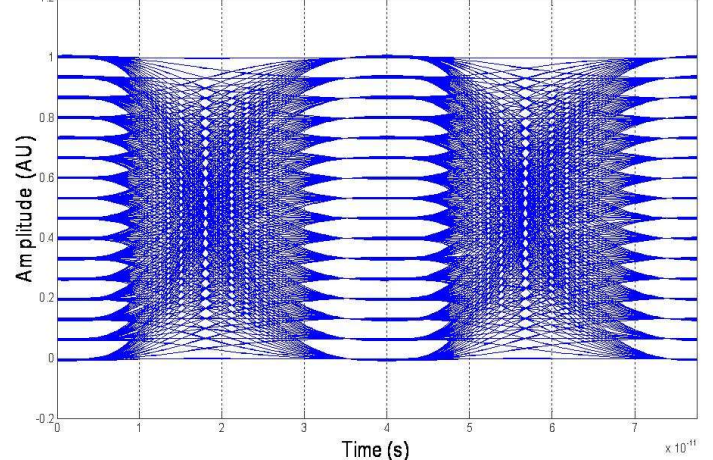
\includegraphics[width=\textwidth]{eye_diagram_pam16.png}
    \caption{Diagram oka PAM16}
    \label{fig:diagram_oka_pam16}
\end{figure}

\subsubsection{PAM --- podsumowanie}

Według artykułu \cite{Higher-order-modulation} przejście z PAM4 na modulacje wyższych rzędów podlega dyskusji. W przypadku PAM4, dwukrotnie większa liczba
poziomów niż w NRZ była opłacalna pomimo mniejszego stosunku sygnału do szumu (SNR). Jednakże przejście z PAM4 na PAM16 nie jest pod tym kątem wydajne, ponieważ
opiera się na bardziej wyrafinowanych technikach odczytu i interpretacji przesyłanych symboli, co wymaga większego zużycia energii.

Z drugiej strony modulacje PAM wyższych rzędów pozwalają na zwiększenie przepustowości w systemach z ograniczoną szerokością pasma --- co
umożliwia implementację technologii wielogigowych w skrętce --- dzięki czemu modulacja PAM16 przyjęła się w standardach 10GBASE-T, 25GBASE-T czy 40GBASE-T.

Te same technologie 10/25/40/50 GbE, które wykorzystują światłowód jako medium, a także technologie 200 GbE i 400 GbE używają NRZ oraz PAM4 z uwagi na prostotę.

\begingroup
\hyphenpenalty10000
\exhyphenpenalty10000
\begin{table}[h]
\captionof{table}{Modulacje w różnych standardach Ethernetowych}
\centering
    \begin{tabular}{m{3cm} m{3cm} m{3cm}}
    \toprule
    Standard & Medium & Modulacja \\
    \midrule
    1000BASE-T & skrętka & PAM5 \\
    \midrule
    1000BASE-T1 & skrętka & PAM3 \\
    \midrule
    1000BASE-KX & światłowód & NRZ \\
    \midrule
    10GBASE-T & skrętka & PAM16 \\
    \midrule
    10GBASE-SR & światłowód & NRZ \\
    \midrule
    25GBASE-T & skrętka & \colorbox{yellow}{PAM16} \\
    \midrule
    25GBASE-SR & światłowód & NRZ \\
    \midrule
    40GBASE-T & skrętka & \colorbox{yellow}{PAM16} \\
    \midrule
    50GBASE-SR & światłowód & PAM4 \\
    \midrule
    100GBASE-ZR & światłowód & PAM4 \\
    \midrule
    200GBASE-SR2 & światłowód & PAM4 \\
    \midrule
    400GBASE-SR4 & światłowód & PAM4 \\
    \bottomrule
    \end{tabular}
\end{table}
\endgroup
